% Author: Izaak Neutelings (June 2020)
% Inspiration:
%   https://www.researchgate.net/figure/a-Refractive-index-and-b-dispersion-of-bulky-soft-glasses-NC21-LLF1-SF6-and-F2-As_fig1_236110630
%   https://link.springer.com/article/10.1007/s11082-014-9979-y
\documentclass[border=3pt,tikz]{standalone}
\usepackage{siunitx}
\usepackage[outline]{contour} % glow around text
\usetikzlibrary{arrows,arrows.meta}
\usetikzlibrary{calc}
\usetikzlibrary{intersections}
\usetikzlibrary{decorations.markings}
\usetikzlibrary{fadings}
\usetikzlibrary{angles,quotes} % for pic (angle labels)
\usetikzlibrary{decorations.pathreplacing} % for curly braces
\usetikzlibrary{decorations.pathmorphing} % for snake lines
\tikzset{>=latex} % for LaTeX arrow head
\contourlength{1.7pt}
\newcommand\degree{^\circ}

\colorlet{myblue}{blue!80!black}
\colorlet{myred}{black!50!red}
\colorlet{watercol}{blue!70!cyan!50}
\tikzstyle{myarr}=[-{Latex[length=3,width=2]}]
\tikzstyle{water}=[ball color=watercol]
\tikzset{
  beam/.style={very thick,line cap=round,line join=round},
  wave/.style={line width=0.2,decorate,decoration={
               snake,pre length=0,post length=0,amplitude=0.1,segment length=#1}},
  wave/.default=2,
}


\begin{document}



% DROPLET refraction & reflection
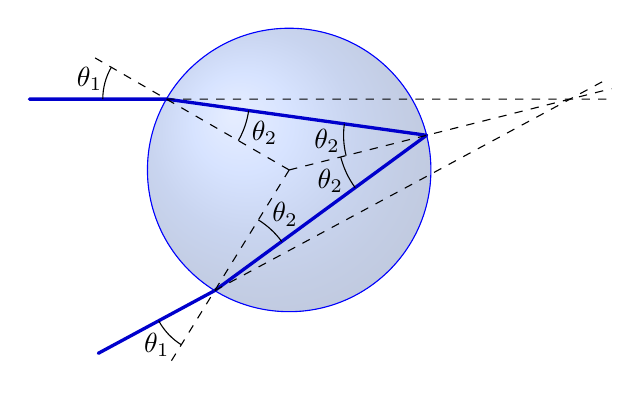
\begin{tikzpicture}
  \def\L{2.4}    % length of ray outside droplet
  \def\R{1.8}    % droplet radius
  \def\na{1.0}   % air
  \def\nw{1.33}  % water
  \def\alphI{150}                                   % A: incident (180-90)
  \pgfmathsetmacro\thetI{180-\alphI}                % theta_1: incident
  \pgfmathsetmacro\thetII{asin(\na/\nw*sin(\thetI)} % theta_2: air -> water & reflection
  \pgfmathsetmacro\alphII{\alphI+2*\thetII-180}     % C: reflected
  \pgfmathsetmacro\alphIII{\alphI+4*\thetII-360}    % D: exiting
  \pgfmathsetmacro\py{\R*sin(\alphI)/sin(\alphII)}  % intersection height
  \coordinate (O) at (0,0);
  \coordinate (A) at (-\L-0.5*\R,{\R*sin(\alphI)});    % incident ray
  \coordinate (B) at (\alphI:\R);                      % entry of incident
  \coordinate (C) at (\alphII:\R);                     % internal reflection
  \coordinate (D) at (\alphIII:\R);                    % exit of ray
  \coordinate (E) at ($(D)+(\alphIII-\thetI:0.7*\L)$); % final ray to observer
  \coordinate (P) at (\alphII:\py);                    % intersection point
  
  % WATER DROPLET
  \fill[water] (O) circle (\R);
  \fill[watercol!20,opacity=0.8] (O) circle (\R);
  \draw[blue] (O) circle (\R);
  
  % LIGHT BEAM
  \draw[beam,myblue] (A) -- (B) -- (C) -- (D) -- (E);
  \draw[dashed] (B) -- (P) --++ (0:0.3*\R);
  \draw[dashed] (O) -- (P) --++ (\alphII:0.3*\R);
  \draw[dashed] (D) -- (P) --++ (2*\alphII:0.3*\R);
  \draw[dashed] (O) -- (B) --++ (\alphI:0.6*\R) coordinate (PB);
  \draw[dashed] (O) -- (D) --++ (\alphIII:0.6*\R) coordinate (PD);
  
  % ANGLES
  \draw pic[-,"$\theta_1$",draw=black,angle radius=23,angle eccentricity=1.25] {angle = PB--B--A};
  \draw pic[-,"$\theta_2$",draw=black,angle radius=30,angle eccentricity=1.25] {angle = O--B--C};
  \draw pic[-,"$\theta_2$",draw=black,angle radius=30,angle eccentricity=1.20] {angle = B--C--O};
  \draw pic[-,"$\theta_2$",draw=black,angle radius=32,angle eccentricity=1.20] {angle = O--C--D};
  \draw pic[-,"$\theta_2$",draw=black,angle radius=30,angle eccentricity=1.25] {angle = C--D--O};
  \draw pic[-,"$\theta_1$",draw=black,angle radius=23,angle eccentricity=1.25] {angle = E--D--PD};
  
\end{tikzpicture}


% DROPLET pileup
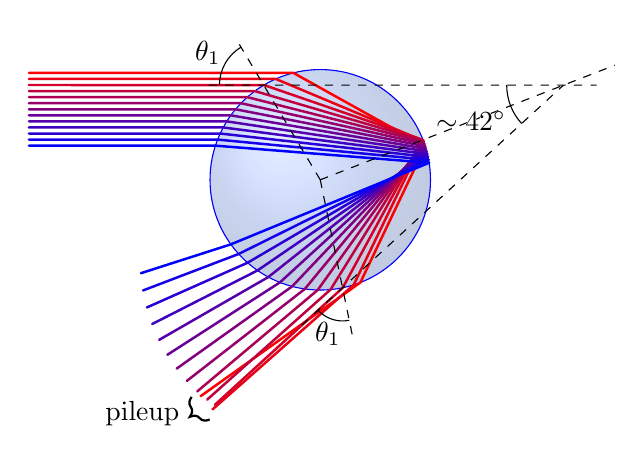
\begin{tikzpicture}
  \def\L{3}      % length of ray outside droplet
  \def\R{1.4}    % droplet radius
  \def\na{1.0}   % air
  \def\nw{1.33}  % water
  \def\N{12}     % number of rays
  \coordinate (O) at (0,0);
  
  % WATER DROPLET
  \fill[water] (O) circle (\R);
  \fill[watercol!20,opacity=0.8] (O) circle (\R);
  \draw[blue] (O) circle (\R);
  
  % LIGHT RAYS
  \foreach \i [evaluate={
      \y=(0.97-\i*0.66/\N)*\R;           % impact parameter
      \alphI=90+acos(\y/\R);             % A: incident (180-90)
      \thetI=180-\alphI;                 % theta_1: incident
      \thetII=asin(\na/\nw*sin(\thetI);  % theta_2: air -> water & reflection
      \alphII=\alphI+2*\thetII-180;      % C: reflected
      \alphIII=\alphI+4*\thetII-360;     % D: exiting
      \f=100-\i*100/\N;                  % color fraction
      \s=0.8-0.4*\i/\N+0.03*int(\y>0.9*\R); % scale
              }] in {0,...,\N}{
    \coordinate (A)   at (-\L-0.5*\R,\y);                 % incident ray
    \coordinate (B)   at (\alphI:\R);                     % entry of incident
    \coordinate (C)   at (\alphII:\R);                    % internal reflection
    \coordinate (D)   at (\alphIII:\R);                   % exit of ray
    \coordinate (E\i) at ($(D)+(\alphIII-\thetI:\s*\L)$); % final ray to observer
    \draw[beam,red!\f!blue,line width=0.9]
      (A) -- (B) -- (C) -- (D) -- (E\i);
  }
  
  % PILEUP
  % https://en.wikipedia.org/wiki/Rainbow#Mathematical_derivation
  % beta = alpI - alpII = 180-2*40.2 = 99.6
  \def\bet{99.6}                                    % alpI - alpII
  \pgfmathsetmacro\thetII{90-\bet/2}                % theta_2: air -> water & reflection
  \pgfmathsetmacro\thetI{asin(\nw/\na*sin(\thetII)} % theta_1: incident
  \pgfmathsetmacro\alphI{180-\thetI}                % A: incident (180-90)
  \pgfmathsetmacro\alphII{\alphI+2*\thetII-180}     % C: reflected
  \pgfmathsetmacro\alphIII{\alphI+4*\thetII-360}    % D: exiting
  \pgfmathsetmacro\py{\R*sin(\alphI)/sin(\alphII)}  % intersection height
  \coordinate (A) at (-\L-\R,{\R*sin(\alphI)});     % incident ray
  \coordinate (B) at (\alphI:\R);                   % entry of incident
  \coordinate (C) at (\alphII:\R);                  % internal reflection
  \coordinate (D) at (\alphIII:\R);                 % exit of ray
  \coordinate (E) at ($(D)+(\alphIII-\thetI:0.5*\R)$); % final ray to observer
  \coordinate (P) at (\alphII:\py);                 % intersection point
  \draw[dashed] (B)++(180:0.5*\R) -- (P) --++ (0:0.3*\R);
  \draw[dashed] (E) -- (D) -- (P); %--++ (0:0.3*\R)
  \draw[dashed] (O) -- (P) --++ (\alphII:0.5*\R);
  \draw[dashed] (O) -- (B) --++ (\alphI:0.5*\R) coordinate (PB);
  \draw[dashed] (O) -- (D) --++ (\alphIII:0.5*\R) coordinate (PD);
  
  % ANGLES
  \draw pic["\strut$\theta_1$",draw=black,angle radius=16,angle eccentricity=1.45] {angle = PB--B--A};
  \draw pic["$\theta_1$",draw=black,angle radius=12,angle eccentricity=1.45] {angle = E--D--PD};
  \draw pic["\contour{white}{$\sim42\degree$}",draw=black,angle radius=20.5,angle eccentricity=1.75] {angle = B--P--D};
  
  % BRACE
  \draw[thick,decorate,decoration={brace,amplitude=5}]
    ($(E2)+(-110:0.2)$) -- ($(E3)+(170:0.2)$) node[black,midway,below=2,left=4] {pileup};
  
\end{tikzpicture}


% DROPLET dispersion & rainbow
\begin{tikzpicture}
  \def\L{1.8}            % length of ray outside droplet
  \def\R{1.6}            % droplet radius
  \def\na{1.0}           % air
  \def\N{6}              % number of rays
  \def\alphI{100}        % A: incident (180-90)
  \pgfmathsetmacro\thetI{180-\alphI} % theta_1: incident
  
  % WATER DROPLET
  \fill[water] (O) circle (\R);
  \fill[watercol!20,opacity=0.8] (O) circle (\R);
  \draw[blue] (O) circle (\R);
  
  % LIGHT RAYS
  \coordinate (O) at (0,0);
  \coordinate (A) at (-\L-\R,{\R*sin(\alphI)}); % incident ray
  \foreach \i [evaluate={
      \lamb=410+\i*320/\N;              % wavelength (for color)
      \nw=1.36-0.08*\i/\N;              % refractive index of water
      \thetII=asin(\na/\nw*sin(\thetI); % theta_2: air -> water & reflection
      \alphII=\alphI+2*\thetII-180;     % C: reflected
      \alphIII=\alphI+4*\thetII-360;    % D: exiting
      \s=0.8+0.45*\i/\N;                % scale
              }] in {0,...,\N}{
    \definecolor{tmpcol}{wave}{\lamb}
    \colorlet{mycol}[rgb]{tmpcol}
    \coordinate (B) at (\alphI:\R);                     % entry of incident
    \coordinate (C) at (\alphII:\R);                    % internal reflection
    \coordinate (D) at (\alphIII:\R);                   % exit of ray
    \coordinate (E) at ($(D)+(\alphIII-\thetI:\s*\L)$); % final ray to observer
    \draw[beam,thick,mycol]
      (B) -- (C) -- (D) -- (E);
  }
  
  % WHITE FADE
  \def\nw{1.30}
  \pgfmathsetmacro\thetII{asin(\na/\nw*sin(\thetI)}
  \draw[myblue,line width=1.3] (A) -- (B);
  \draw[beam,white,line width=1.0] (A) -- (B);
  %\draw[beam,white,line width=1.0,path fading=east] (B) --++ (-180+\alphI+\thetII:0.01);
  \draw[beam,white,line width=1.0,path fading=east] (B) --++ (-180+\alphI+\thetII:0.6*\R);
  %\draw[beam,white,line width=1.2] (B)++(-0.005,0) -- (B) --++ (-180+\alphI+\thetII:0.005);
  
\end{tikzpicture}


% GRADIENT RAINBOW
% Instead of smooth gradient, use many thin polygons
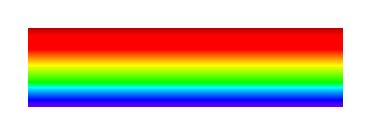
\begin{tikzpicture}
  \def\H{1} % width of band
  \def\L{4} % length of rays
  \def\N{200}
  \foreach \i [evaluate={\f=\i/\N; \lamb=410+\f*320;\y=\f*\H;}] in {0,...,\N}{
    \definecolor{tmpcol}{wave}{\lamb}
    \colorlet{mycol}[rgb]{tmpcol}
    \draw[mycol,line width=0.3] (0,\y) -- (\L,\y);
  }
\end{tikzpicture}


% GRADIENT RAINBOW - divergent
% Instead of smooth gradient, use many thin polygons
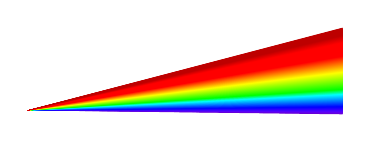
\begin{tikzpicture}
  \def\H{1} % width of band
  \def\L{4} % length of rays
  \def\N{200}
  \foreach \i [evaluate={\f=\i/\N; \lamb=410.+\f*320.;\y=\f*\H;}] in {0,...,\N}{
    \definecolor{tmpcol}{wave}{\lamb}
    \colorlet{mycol}[rgb]{tmpcol}
    %\draw[beam,thick,mycol] (0,\y) -- (\L,\y);
    \fill[mycol,line width=0.3] (0,0) -- (\L,\y+0.05) -- (\L,\y-0.05) -- cycle;
  }
\end{tikzpicture}



\end{document}